% Architecture-as-equation figure for the shielding-tensor model (Stage 3, Model 1).
% The point: the network IS the unifying equation  sigma_ab(i) ~ sum_s I_s D_ab(r_is).
% One shared e3nn angular block = the kernel D_ab; a per-type radial MLP = the intensity I_s.
% Output is a rank-2 tensor (T2), never a scalar.  Compile: pdflatex -interaction=nonstopmode
\documentclass[border=12pt]{standalone}
\usepackage{amsmath}
\usepackage{tikz}
\usetikzlibrary{positioning,arrows.meta,fit,backgrounds,calc,shapes.geometric}

\definecolor{ink}{RGB}{40,64,98}
\definecolor{cAng}{RGB}{205,221,240}
\definecolor{cRad}{RGB}{243,228,198}
\definecolor{cPool}{RGB}{231,231,234}
\definecolor{cOut}{RGB}{205,229,210}
\definecolor{cIn}{RGB}{246,246,248}
\definecolor{note}{RGB}{116,116,126}

\begin{document}
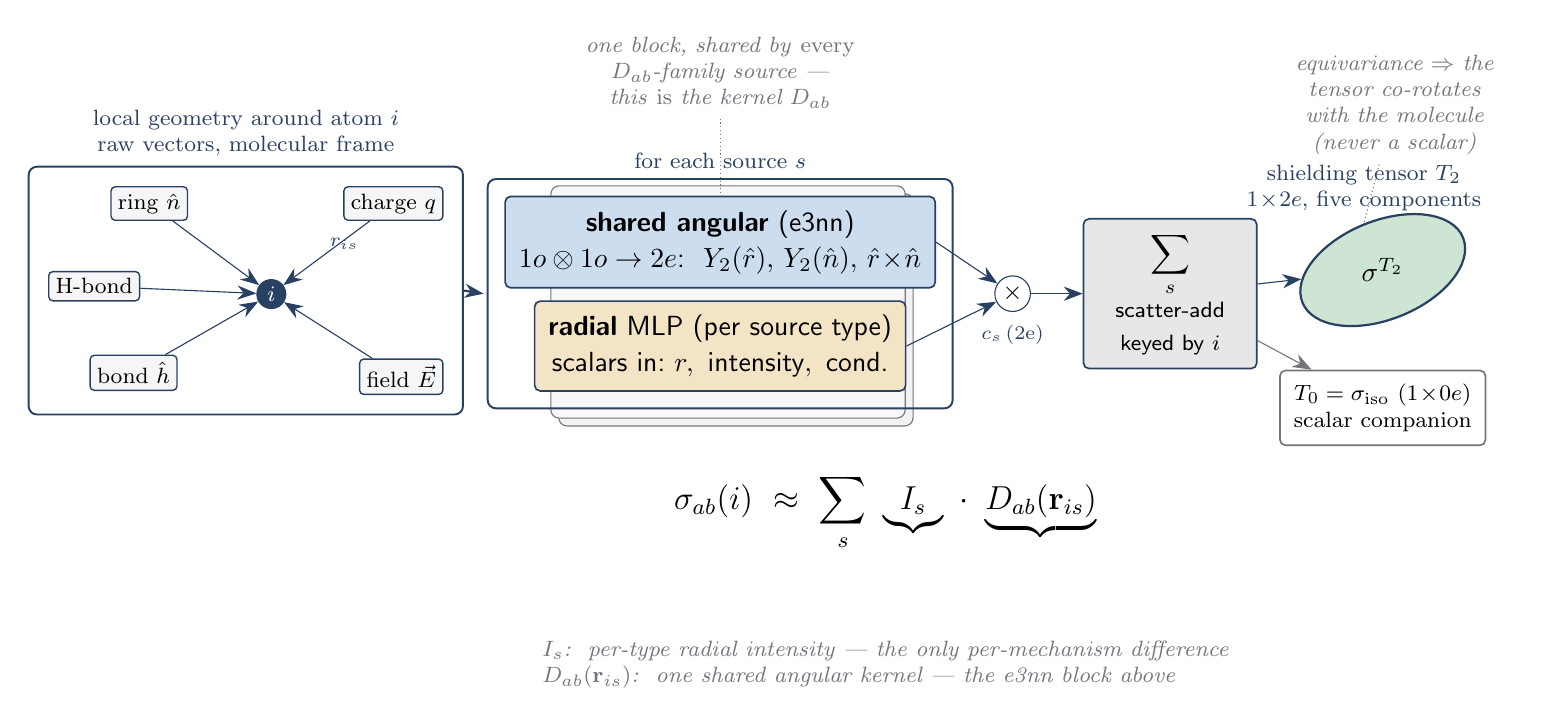
\begin{tikzpicture}[
  font=\sffamily,
  >={Stealth[length=2.4mm]},
  blk/.style={rounded corners=2pt, draw=ink, line width=0.6pt, align=center, inner sep=5pt, fill=white},
  src/.style={draw=ink, line width=0.5pt, fill=cIn, rounded corners=1.5pt, inner sep=2.5pt, font=\footnotesize},
  lead/.style={draw=note, line width=0.4pt, densely dotted},
  ntxt/.style={text=note, font=\footnotesize\itshape, align=center},
  lab/.style={font=\footnotesize, text=ink}
]

% ---------------- INPUT: local geometry around atom i ----------------
\node (i) at (0,0) [circle, draw=ink, fill=ink, text=white, inner sep=1.6pt, font=\footnotesize] {$i$};
\node (s_ring) at (-1.55,1.15) [src] {ring $\hat{n}$};
\node (s_q)    at (1.55,1.15)  [src] {charge $q$};
\node (s_bond) at (-1.75,-1.0) [src] {bond $\hat{h}$};
\node (s_fld)  at (1.65,-1.05) [src] {field $\vec{E}$};
\node (s_hb)   at (-2.25,0.1)  [src] {H-bond};
\draw[->,ink] (s_ring) -- (i);
\draw[->,ink] (s_q) -- (i) node[midway,above right,lab,font=\scriptsize,inner sep=1pt] {$r_{is}$};
\draw[->,ink] (s_bond) -- (i);
\draw[->,ink] (s_fld) -- (i);
\draw[->,ink] (s_hb) -- (i);
\node[fit=(s_ring)(s_q)(s_bond)(s_fld)(s_hb)(i), rounded corners=3pt, draw=ink, line width=0.7pt, inner sep=7pt] (inbox) {};
\node[above=0pt of inbox, lab, align=center] {local geometry around atom $i$\\{\footnotesize raw vectors, molecular frame}};

% ---------------- PER-SOURCE UNIT ----------------
\coordinate (cB) at (5.7,0);
\begin{scope}[on background layer]
  \node[rounded corners=3pt, fill=cPool!55, draw=note, line width=0.4pt] at ($(cB)+(0.20,-0.20)$) [minimum width=4.5cm, minimum height=2.95cm] {};
  \node[rounded corners=3pt, fill=cPool!30, draw=note, line width=0.4pt] at ($(cB)+(0.10,-0.10)$) [minimum width=4.5cm, minimum height=2.95cm] {};
\end{scope}
\node (ang) at ($(cB)+(0,0.66)$) [blk, fill=cAng, minimum width=4.1cm] {\textbf{shared angular} (e3nn)\\[1pt]$1o\otimes 1o\to 2e$:\ \ $Y_2(\hat r),\,Y_2(\hat n),\,\hat r\!\times\!\hat n$};
\node (rad) at ($(cB)+(0,-0.66)$)[blk, fill=cRad, minimum width=4.1cm] {\textbf{radial} MLP\ (per source type)\\[1pt]scalars in:\ $r,\ \text{intensity},\ \text{cond.}$};
\node[fit=(ang)(rad), rounded corners=3pt, draw=ink, line width=0.7pt, inner sep=6pt] (unit) {};
\node[above=0pt of unit, lab] {for each source $s$};

\node (mul) at ($(unit.east)+(0.75,0)$) [circle, draw=ink, fill=white, inner sep=1.2pt, font=\small] {$\times$};
\node[below=1pt of mul, lab, font=\scriptsize] {$c_s$\,(2e)};
\draw[->,ink] (ang.east) -- (mul);
\draw[->,ink] (rad.east) -- (mul);
\draw[->,ink, line width=0.8pt] (inbox.east) -- ($(unit.west)+(-0.04,0)$);

% ---------------- POOL ----------------
\node (pool) at ($(mul)+(2.0,0)$) [blk, fill=cPool, minimum width=2.2cm] {$\displaystyle\sum_s$\\[1pt]{\footnotesize scatter-add}\\{\footnotesize keyed by $i$}};
\draw[->,ink] (mul) -- (pool);

% ---------------- OUTPUT ----------------
\node (glyph) at ($(pool)+(2.7,0.30)$) [draw=ink, fill=cOut, ellipse, minimum width=2.2cm, minimum height=1.25cm, line width=0.8pt, rotate=22] {};
\node at (glyph) {$\sigma^{T_2}$};
\node[above=1pt of glyph, lab, align=center] {shielding tensor $T_2$\\{\footnotesize $1\!\times\!2e$, five components}};
\node (t0) at ($(pool)+(2.7,-1.45)$) [blk, fill=white, draw=note, font=\footnotesize] {$T_0=\sigma_{\mathrm{iso}}$\ ($1\!\times\!0e$)\\ scalar companion};
\draw[->,ink] (pool) -- (glyph);
\draw[->,note] (pool) -- (t0);

% ---------------- EQUATION BANNER ----------------
\node (eq) at ($(cB)+(2.1,-3.0)$) [font=\large] {$\displaystyle \sigma_{ab}(i)\ \approx\ \sum_{s}\ \underbrace{I_s}_{\strut}\ \cdot\ \underbrace{D_{ab}(\mathbf r_{is})}_{\strut}$};
\node[below=0.45cm of eq, ntxt, align=left] {$I_s$:\ \ per-type radial intensity --- the only per-mechanism difference\\$D_{ab}(\mathbf r_{is})$:\ \ one shared angular kernel --- the e3nn block above};

% ---------------- CALLOUTS ----------------
\node[ntxt, text width=3.5cm] (cAngN) at ($(ang)+(0,2.15)$) {one block, shared by \emph{every} $D_{ab}$-family source --- this \emph{is} the kernel $D_{ab}$};
\draw[lead] (cAngN) -- (ang.north);
\node[ntxt, text width=3.3cm] (cOutN) at ($(glyph)+(0.15,2.1)$) {equivariance $\Rightarrow$ the tensor co-rotates with the molecule (never a scalar)};
\draw[lead] (cOutN) -- (glyph.north);

\end{tikzpicture}
\end{document}
